


%In this chapter you should describe the previous (if possible) and final experiments performed on the implementation.

%Every single experiment should be explained individually, providing to the reader information about the meaning of the experiment, the expected (theoretical) results, the final results, the comparison between them and others (if possible) and the conclusions. 

%Each experiment should include a description, covering (when possible) the following information:
%\begin{itemize}
% \item Significant physical features (obstacles present on the environment, human presence, temperature, humidity, possible noise sources, computational speed of the machine, etc.)
% \item The precise location of the experiment (latitude and longitude, room number or citation to a description of the used laboratory).
% \item Sampling design (variable(s) measured, transformation performed to the data, samples collected, replication, comparative with a Ground Truth system, collecting data protocol).
% \item Analysis design (how the data are processed, statistical procedures used, statistical level to determine significance).
%\end{itemize}
%The provided information should be sufficient to allow other scientists to repeat your experiment in the same conditions. Thus, the use of standard and well-known equipment could only be represented by a simple sentence, but the non-standard equipment should be described in detail, citing the source (vendor) and most important characteristics.

%To write it, try to use the third person when describing the experiments and results. Avoid to use first person. Past tense should be the dominant conjugation (the work is done and was performed in the past).

%Note: Graphics represent really well data, use them! (Matlab or Octave could be useful for that).

\chapter{Evaluation}
\label{ch:evaluation}

\section{Simulation}

\subsection{Sensor Simulation}


\subsection{Office Environment}

\section{Experiment Procedure}

\subsection{Gather Information Experiment}

\subsection{Navigation Experiment}

\section{Experiment Summery}



This chapter introduces the experiments performed on the implementation. 
Chapter \ref{sec:experiment_set_up} presents precondition of experiments.
Chapter \ref{sec:sensor_simulatior} introduces the simulated sensors.
Chapter \ref{sec:gather_info_task_experiments} presents the experiments in the case that the centralized pool assign only ``gather information tasks'' to robots.
Chapter \ref{sec:execute_task_experiments} presents the experiment in the case that centralized pool assign only ``navigation tasks'' to robots. 


\section{Experiment Setup}

There following are some preparation before performing experiments. 
\label{sec:experiment_set_up}
\begin{enumerate}
\item \textbf{Create a Launch file for Simulation} Create a launch file. Firstly this file loaded a gazebo world model with an office environment (Figure \ref{fig:gazebo_model}). In this environment, the start time should set to ``2020-06-01 9:00:00''. Secondly, it loaded three robot models as well as robot state publishers to simulates robot activity such as LDR sensor measurement.
\begin{figure}[htbp]
 \centering
 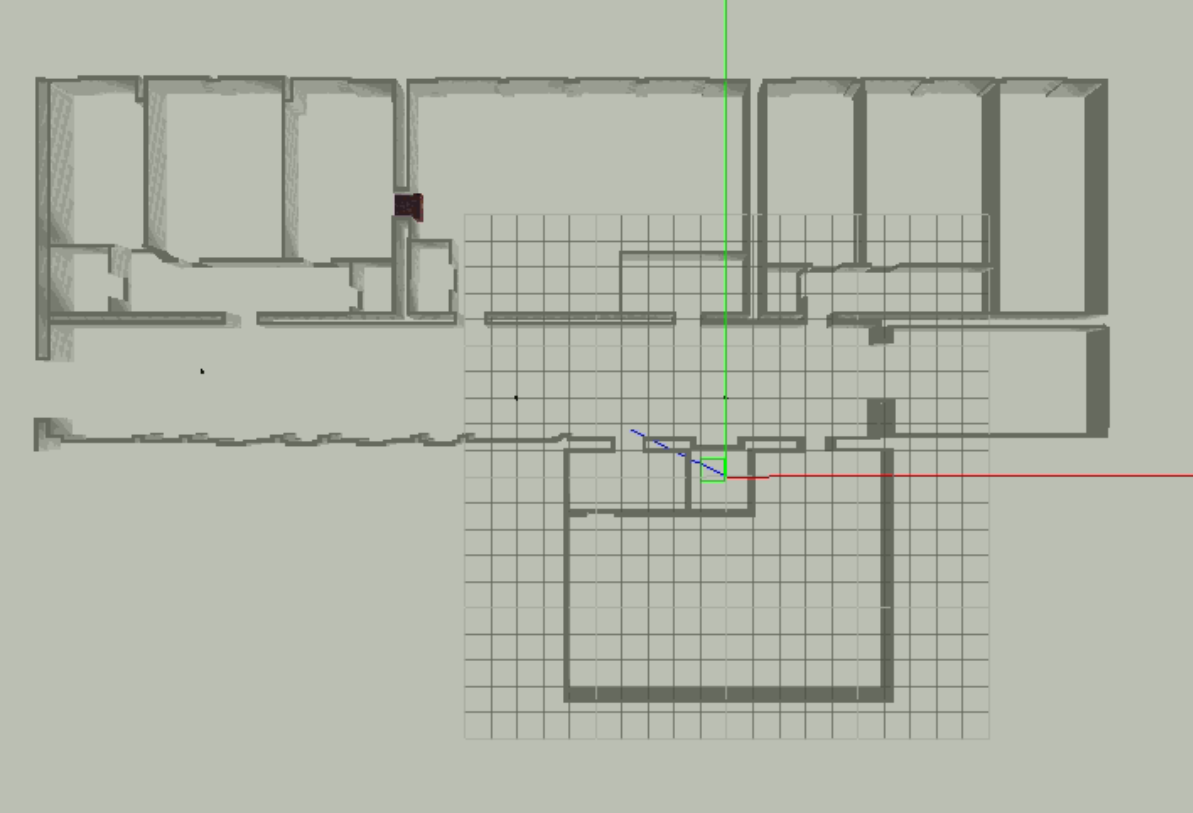
\includegraphics[width = 0.7\textwidth]{content/images/ch5/gazebo_model.png}
 \caption{Gazebo Simulation}
 \label{fig:gazebo_model}
\end{figure}

\item \textbf{Create a Launch file for Navigation Stack.} Create the second launch file. This file started the navigation stack (move\_base node). It also started map server to load the map (Figure \ref{fig:exp_map}) created by SLAM\cite{T3SLAM} and open the GUI of Rviz.  
\begin{figure}[htbp]
 \centering
 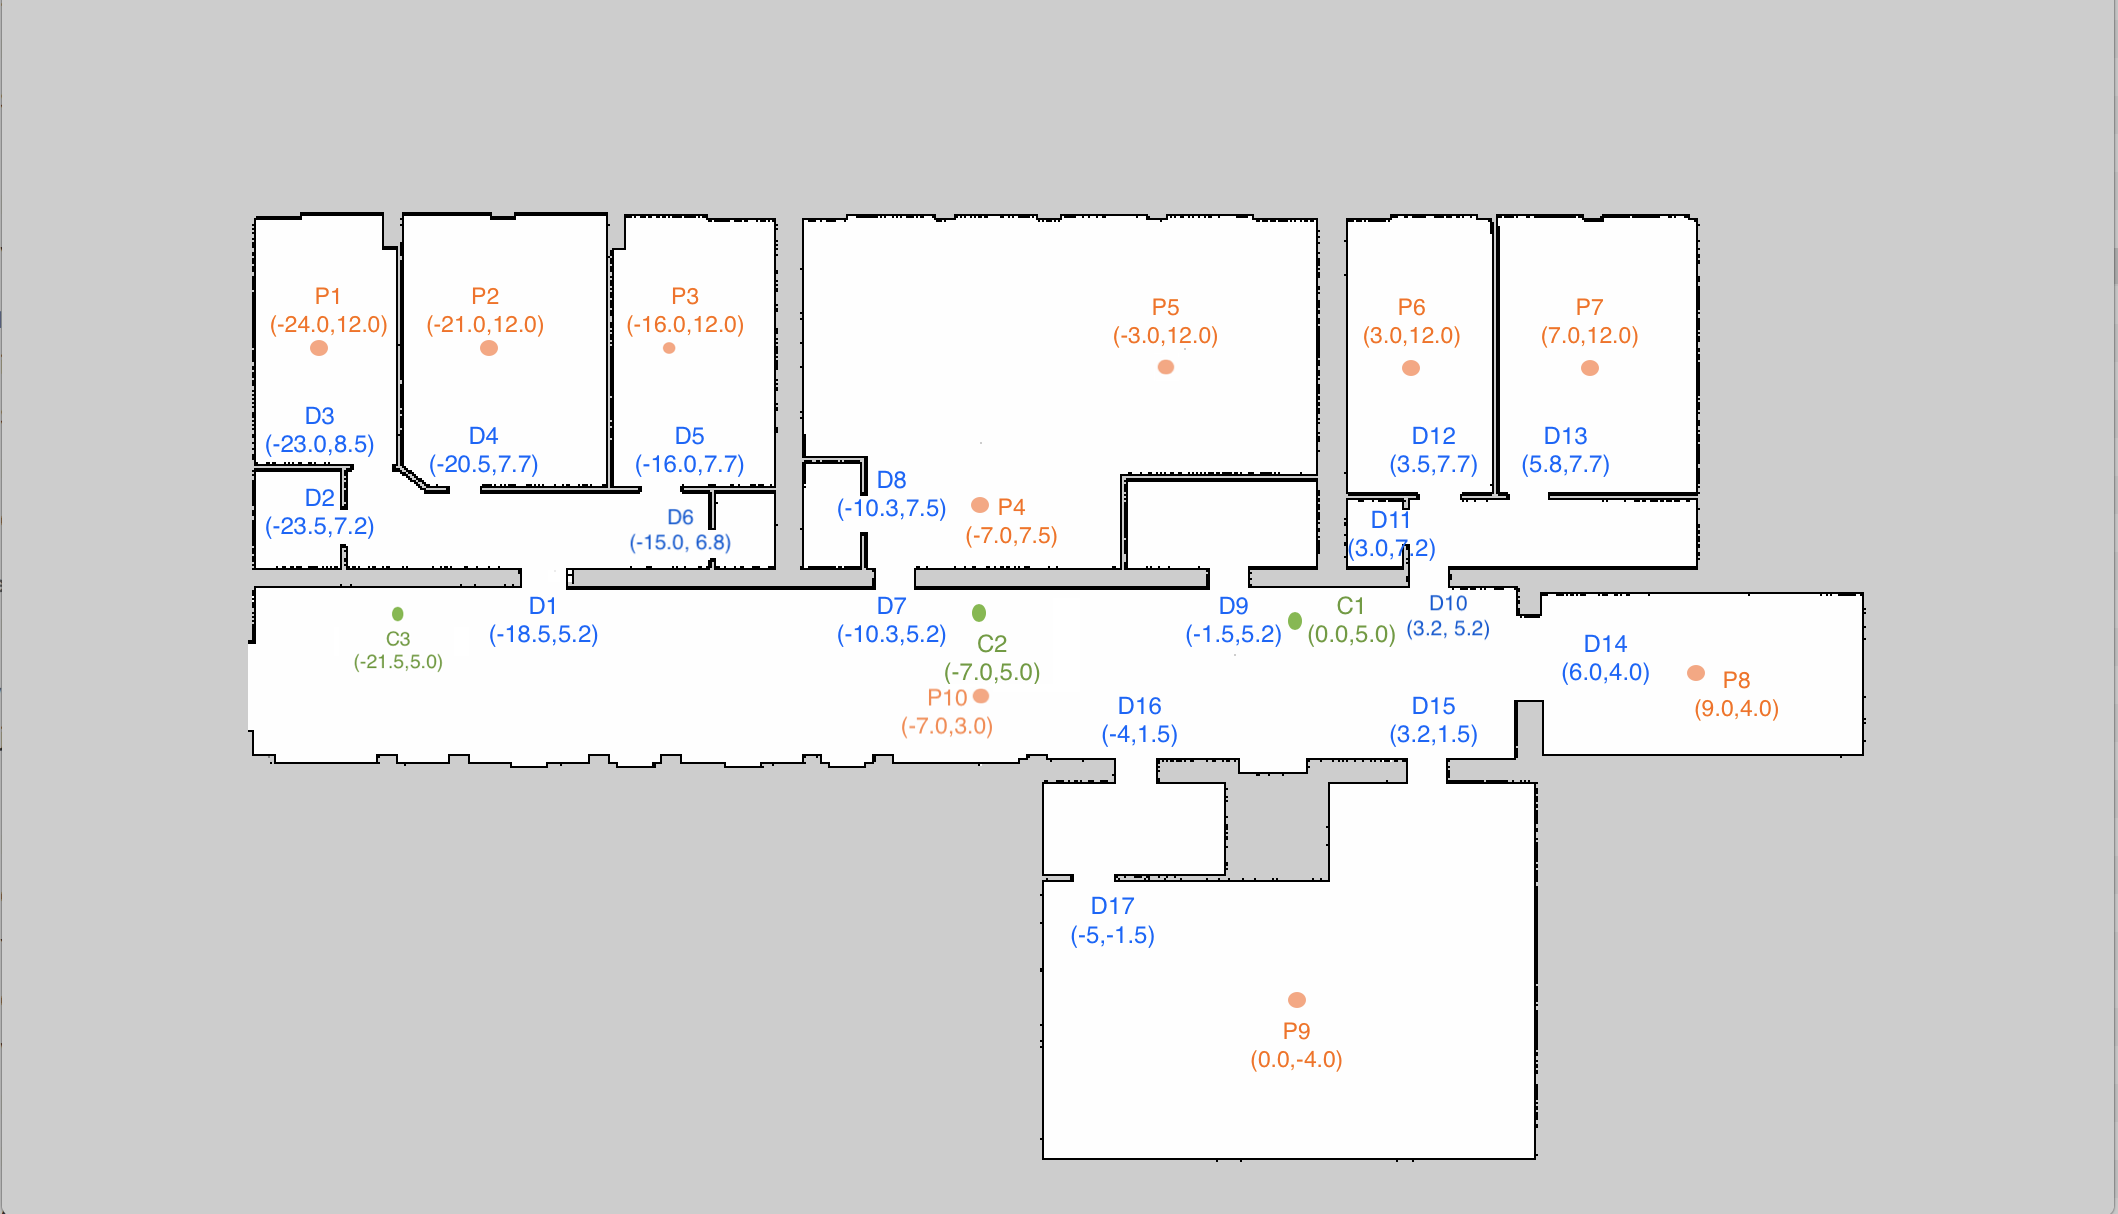
\includegraphics[width = 0.9\textwidth]{content/images/ch5/door_station_points.png}
 \caption{Experiment Map.}
 \label{fig:exp_map}
 \end{figure}

 \item \textbf{Create a Launch file for ROS nodes.} Create the third launch file to start ROS node ``centralized pool'',``robot controller'', ``sensor simulator'' and ``charging station''. 
 \item \textbf{Configure MySQL database.} Start MySQL database server on the computer and start the charging event in the database.
 \item \textbf{Design the database script to gather information experiment.} The script of gather information experiment is shown in Figure \ref{fig:env_exp_timeline}. This script had the following advantages. The first advantage was that this script prevented the initial position from affecting the experiment results. At the beginning of each experiment, all robots started from their initial position, which is the charging station. The second advantage was that the robot would charge after each experiment. This script ensures that the robot would not stop moving due to a lack of energy during the experiment. The third advantage was that each robot gathered the information for time T in each experiment. After an experiment with T set to 15 minutes, about 200 measurement data and 40 task results would be gathered and stored in the database. 
 \begin{figure}[htbp]
 \centering
 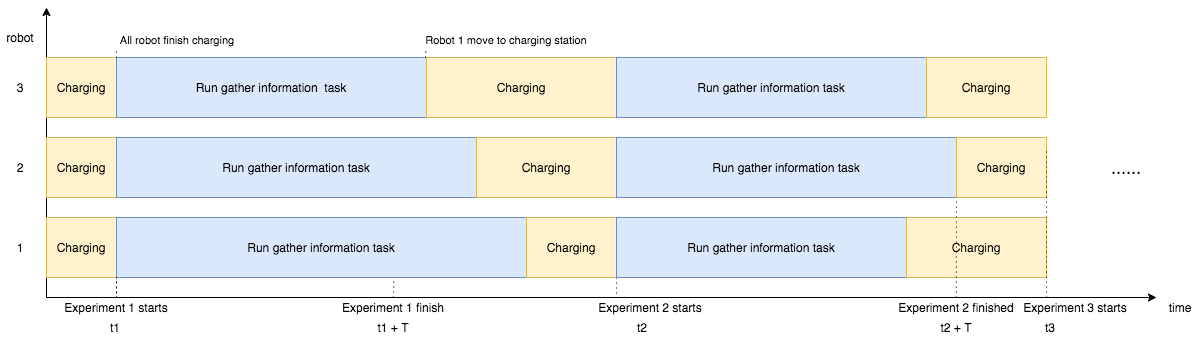
\includegraphics[width = 0.7\textwidth]{content/images/ch5/env_exp_timeline.drawio.png}
 \caption{The script of gather information experiment.}
 \label{fig:env_exp_timeline}
 \end{figure}

 \item \textbf{Design the database script to navigation experiment.} The script of gather information experiment is shown in Figure \ref{fig:nav_exp_timeline}.
 This script had the following advantages. The first advantage was that this script prevented the initial position from affecting the experiment results. At the beginning of each experiment, all robots started from their initial position, which was the charging station. The second advantage was that the robot would charge after each experiment. This script ensured that the robot would not stop moving due to a lack of energy during the experiment. The third feature is that 15 navigation tasks with equal time intervals in each experiment will be generated. The number of successful tasks and the completion time of all tasks will be used to evaluate task scheduling performance.
 Table \ref{tab:exp_task_table} shows ``task table'' in database. At this point, robots finished task 4-21 in experiment 1 and finished 21-39 in experiment 2. 
 \begin{figure}[htbp]
 \centering
 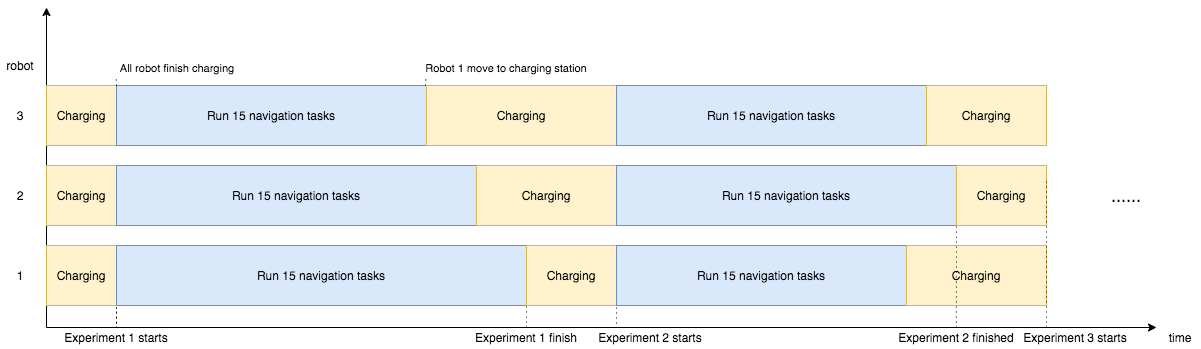
\includegraphics[width = 0.7\textwidth]{content/images/ch5/exe_exp_timeline.drawio.png}
 \caption{The script of navigation experiment.}
 \label{fig:nav_exp_timeline}
 \end{figure}
\item \textbf{Connect the corresponding database script to the centralized pool.} When the centralized pool found that the current experiment should end, it should run the database script to automatically start the next experiment.
\item \textbf{Set up experiment condition.} The weight values should be import to ``experiment result'' in database
\item \textbf{Run the launch file.} After setting up, the user should run the three launch file. The experiment would keep running until all entities in ``experiment result'' table was filled.


\end{enumerate}




\section{Sensor Simulator}
\label{sec:sensor_simulatior}

\paragraph{Sensor Message Publish}
In this project, a sensor simulator node is used to publish measurement results. The door simulator publishes one message for each door periodically to a ROS topic ``sensor data''. The message contains door id, sensor position and door status(Table \ref{sec:measurement_message}). The door status are created according to open possibilities table (Table \ref{tab:db_open_possibilities}). 


\paragraph{Generate Measuring Data}
For example, on monday (day of week is 2) at simulation time ``10:30:00'' (on time slot 10:00:00-10:59:59), in 80\% probability a ``door open'' is generated and in 20\% a ``door closed'' is generated (Initialized Open Possibility is 0.80).


\paragraph{Sensor Message Subscribe}
The process of sensor simulation is shown in Figure \ref{sec:sensor_simulatior}. The robots (robot controller nodes) subscribe to the same ROS topic ``sensor data''. Every time the sensor simulator sends a message, all robots will receive this message simultaneously. Their distance filters filter sensor messages with a position outside the communication range and keep sensor messages within the communication range. With this process, the sensor simulator sends the instant measurement result to robots within the communication range. However, if the system is applied to the real world, the real-world sensor could send a record with history measurement instead of sending instant measurement data.

\begin{figure}
\centering
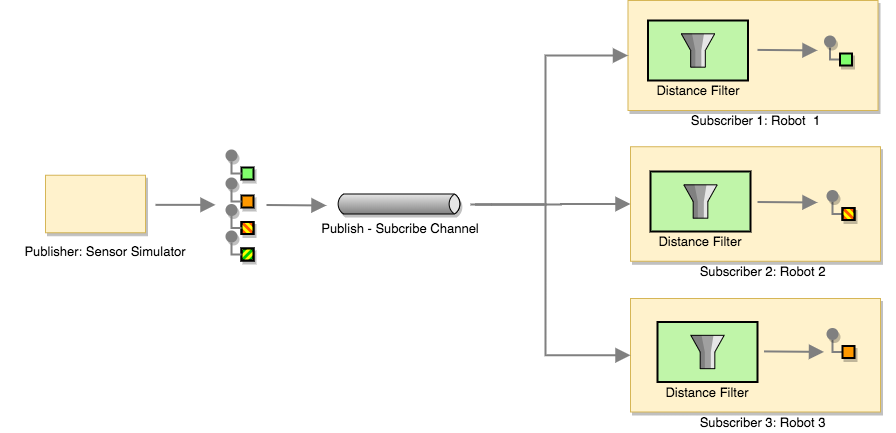
\includegraphics[width = 0.7\textwidth]{content/images/ch4/sensor_simulator.drawio.png}
\caption{Sensor Simulator}
\label{fig:sensor_simulator}
\end{figure}

\section{Gather Information Task Experiment Result}
\label{sec:gather_info_task_experiments}

\subsection{Use Enumeration Method to Find the Best Weight Combinations}
\label{sec:gather_info_experiment_enumerate}
\paragraph{Experiment Introduction} 
To find the best weight combinations, 30 experiment are created with $W_{\mbox{energy consumption}} \in \{ 0,1,5,10 \}, W_{\mbox{update}} \in \{-10,-5,-1\}, W_{\mbox{probability}} \in \{-10,-5,-1,0\}$. In addition, the conditions $W_{\mbox{update}}=0$ was not testable, because during the experiment centralized pool generate the same ``gather information tasks``, which let robots not moving and measuring their nearest door. Experiment Duration T = 10 min.


\paragraph{Analysis design} The experiment start time was when all robot finished charging and started request task (Figure \ref{fig:env_exp_timeline}). The experiment duration is a constant value T. The experiment finish time $T_{\mbox{finish time}} = T_{\mbox{start time}} + T $. Some important factors are evaluated. 

\begin{itemize}
 \item \textbf{Last Update.} The ``last update'' factor is the time difference between experiment start time and minimal value in ``last update'' column in door table (Table \ref{tab:db_doors}) when an experiment finished. For example, ``last update'' factor in experiment 1 (Figure \ref{fig:gather_info_experiment_enumerate}) is ``00:02:57''. It means that the door in the worst case not be measured since 2 minutes 57 seconds after experiment start.
 \item \textbf{Average Update Interval} The ``Average update interval'' means the average interval of door update. For example, ``Average Update Interval'' factor in experiment 1 (Figure \ref{fig:gather_info_experiment_enumerate}) is ``00:01:00''. It means that on average, every door is updated every minute.
 \item \textbf{Succeeded Task.} The ``Number of task'' factor means the number of succeeded ``gather information'' task.
\end{itemize}

\paragraph{Experiment Result} 
Figure \ref{fig:gather_info_experiment_enumerate} represent the experiment result.

\paragraph{Experiment Analysis} 

As shown in the experiment result, all ``Minimal Last Update'' value is from 1 min to 5 min, much less than the experiment duration (10 min). It means some doors were not timely updated information. One possible reason is that the velocity of the robot is small (about 0.2 per second). The experiment duration (10min) was not long enough to let three robots pass to all doors. Another possible reason is that the robot's route is partially duplicated. For example, when the system started, robot 1 was at charging station 1 and got a task to door 3, while robot 2 was at charging station 2 and got a task to door 4. As shown in Figure \ref{fig:positions_door_station}, these two route are partially duplicated, both of them pass through door 1 and entered room 1 (Figure \ref{fig:room_division}). The ideal solution was to give both tasks to one robot. 

\begin{figure}[htbp]
 \centering
 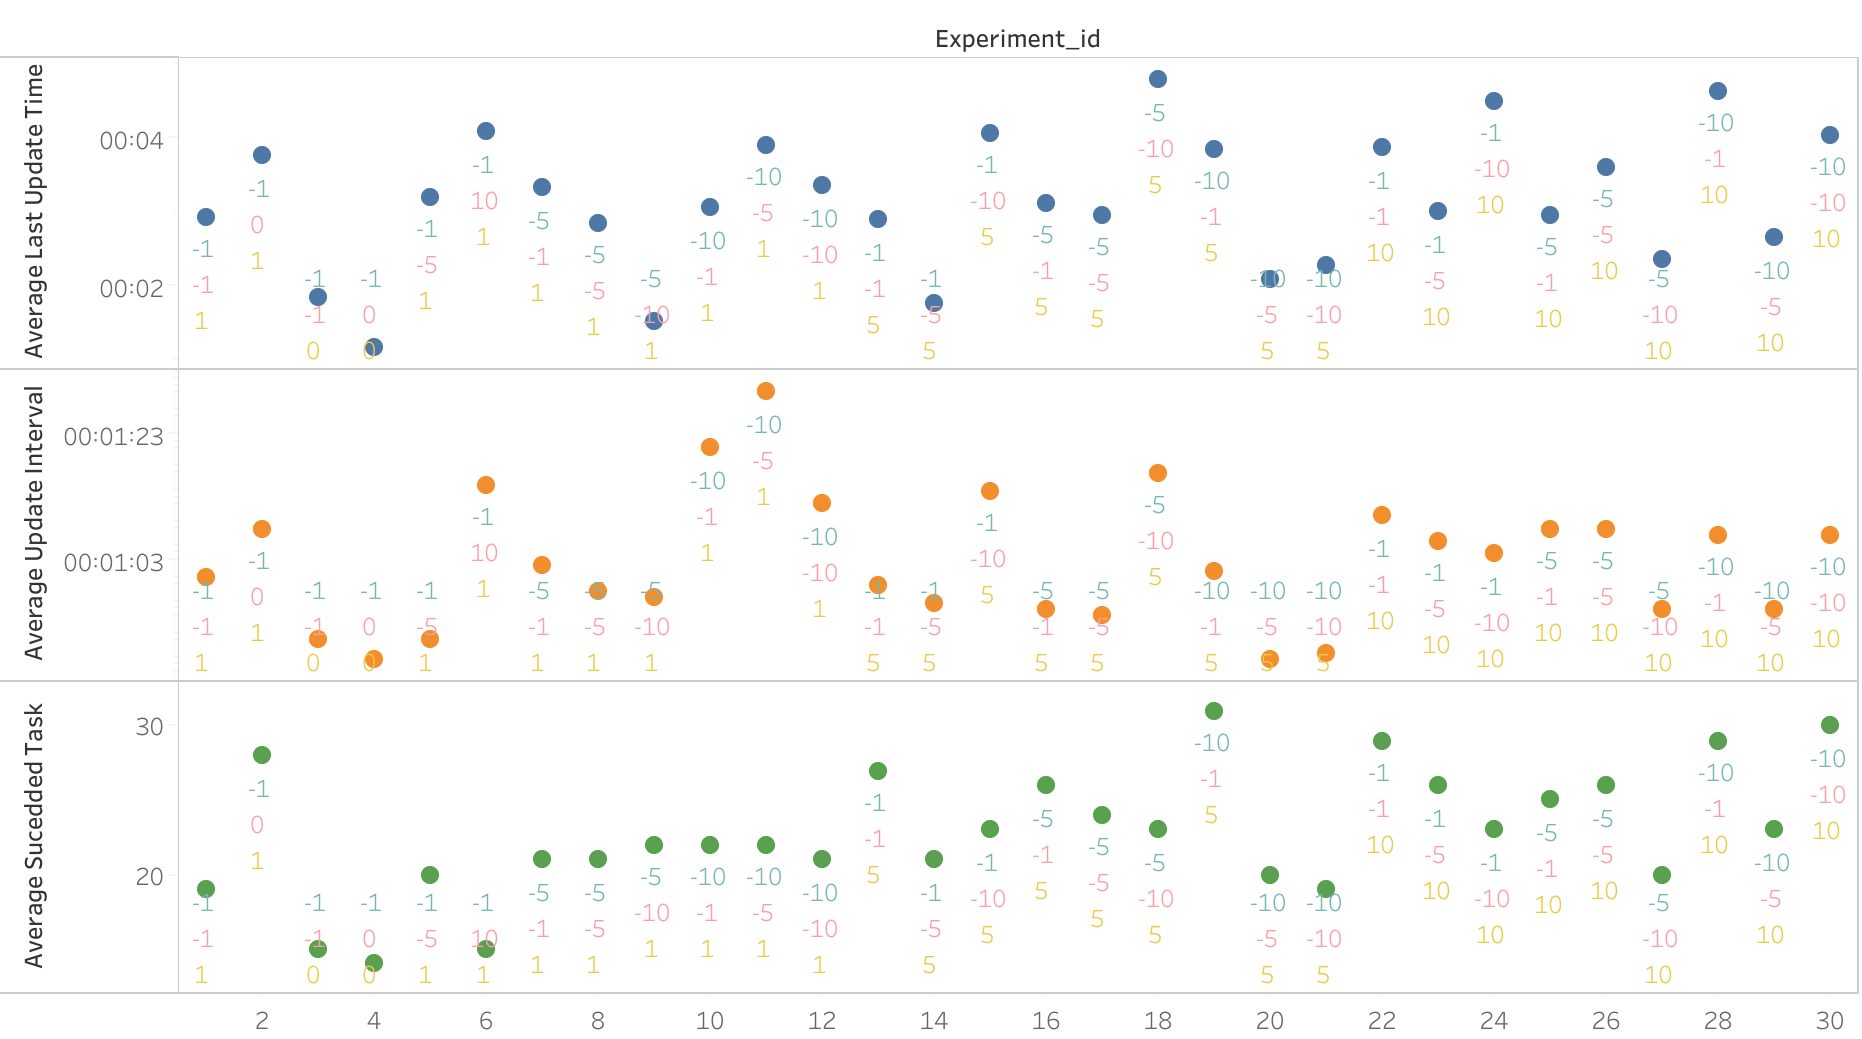
\includegraphics[width = 0.9\textwidth]{content/images/ch5/gather_info_enumerate.png}
 \caption{Experiment: Use enumeration method to find best weight combination}
 \text{Green: $W_{\mbox{battery}}$ Pink: $ W_{\mbox{probability}}$ Yellow: $W_{\mbox{update}} $}
 \label{fig:gather_info_experiment_enumerate}
\end{figure}


\subsection{Use Analysis to Find the Best Weight Combinations}

\paragraph{Experiment Introduction} 
As is discussed in the last experiment (Chapter \ref{sec:gather_info_experiment_enumerate}), the experiment time was too short to allow the robot to explore each door. Therefore, the experiment duration in this experiment was increased to 20 min.
Firstly, we should find the best weight combination for ``weight battery'' and ``weight last update'', then find the third weight ``weight probability''. Finally, the best combination of weight will be concluded.
 According to the cost table (Figure \ref{fig:cost_table}), the update time value has a minimal value of 6.986 and a maximal value of 336.986 (column 3), which are much larger than energy consumption (column 2) and product of door open possibilities (column 4).
 Therefore, 18 experiments are created with $W_{\mbox{battery}}$
 = 0.1 and $W_{\mbox{battery}} \in \{1,5,10,15,20,25 \}$.

\paragraph{Analysis design} The experiment start time was when all robot finished charging and started request task (Figure \ref{fig:env_exp_timeline}). The experiment duration is a constant value T. The experiment finish time $T_{\mbox{finish time}} = T_{\mbox{start time}} + T $. Some important factors are evaluated. 
\begin{itemize}
 \item \textbf{Last update.} The ``last update'' factor is the time difference between experiment start time and minimal value in ``last update'' column in door table (Table \ref{tab:db_doors}) when an experiment finished. For example, ``last update'' factor in experiment 1 (Figure \ref{fig:gather_info_experiment_enumerate}) is ``00:02:57''. It means that the door in the worst case not be measured since 2 minutes 57 seconds after experiment start.
 \item \textbf{Average Update Interval} The ``Average update interval'' means the average interval of door update. For example, ``Average Update interval'' factor in experiment 1 is ``00:01:00''. It means that on average, every door is updated every 1 minute.
 \item \textbf{Succeeded task.} The ``Number of task'' factor means the number of succeeded ``gather information'' task.
\end{itemize}

\begin{figure}[htbp]
 \centering
 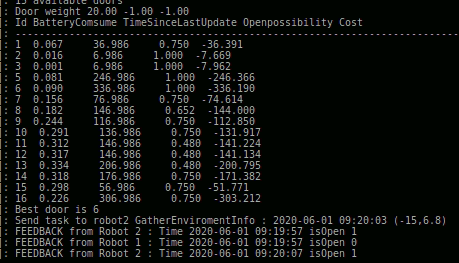
\includegraphics[width = 0.7\textwidth]{content/images/ch5/weight_analyze.png}
 \caption{Centralized Pool Cost Table}
 \label{fig:cost_table}
\end{figure}

\paragraph{Experiment Result} The experiment results are shown in Figure \ref{fig:gather_info_experiment_two_value} and Figure \ref{fig:gather_info_experiment_three_value}
\begin{figure}[htbp]
 \centering
 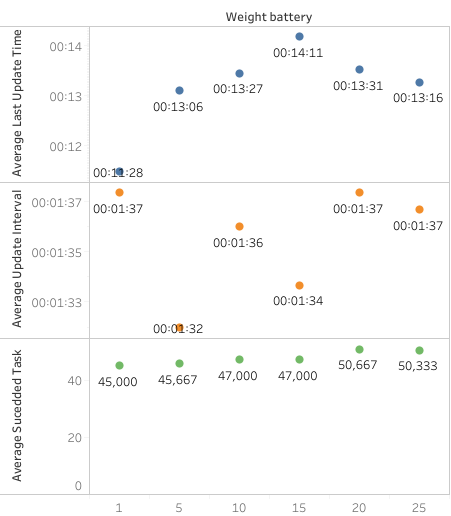
\includegraphics[width = 0.7\textwidth]{content/images/ch5/gather_info_change_weight_battery_only.png}
 \caption{Experiment: Change $W_{\mbox{battery}}$ under condition $W_{\mbox{update}} = 0.1$ and $W_{\mbox{probability}}=0$}
 \label{fig:gather_info_experiment_two_value}
\end{figure}

\begin{figure}[htbp]
 \centering
 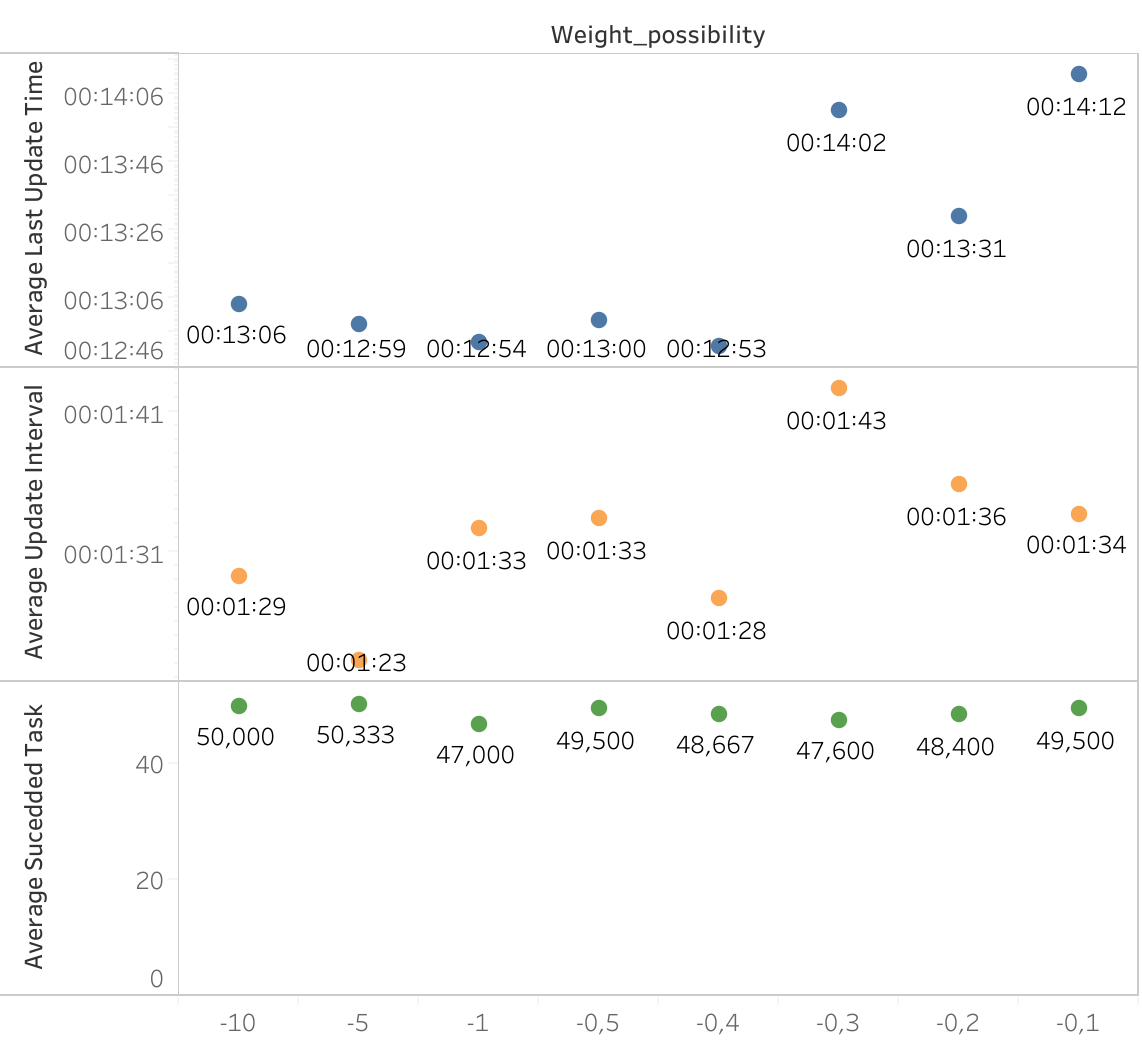
\includegraphics[width = 0.7\textwidth]{content/images/ch5/gather_info_change_weight_probability_only.png}
 \caption{Experiment: Change $W_{\mbox{probability}}$ under condition $W_{\mbox{battery}}=15$ and $ W_{\mbox{update}}=0.1$}
 \label{fig:gather_info_experiment_three_value}
\end{figure}

\paragraph{Experiment Analysis} 
As shown in experiment result Figure \ref{fig:gather_info_experiment_two_value}, ``weight battery'' increased from 0 to 25, the ``average succeeded experiment task number'' slightly increased from 45 to 50, but ``average update interval'' were floated in a small range around ``00:01:35''. Especially, as ``weight battery'' increased from 0 to 15, ``average last update'' showed an upward trend, and as ``weight battery'' increased from 15 to 25, ``average last update'' showed a downward trend, 
therefore ``weight battery'' 15 and ``weight update'' 0.1 was the best combination. 
This combination was used in next experiment set (Figure \ref{fig:gather_info_experiment_three_value}). From this experiment set, it was concluded that ``weight battery'' 15, ``weight update'' 0.1, ``weight probability'' 0.1 and ``weight battery'' 15, ``weight update'' 0.1, ``weight probability'' -0.3 were two best weight combinations for the cost function.

\section{Execute Task Evaluation Experiment}
\label{sec:execute_task_experiments}


\subsection{Experiment: Find the Best Weight Combinations}
\paragraph{Experiment Introduction}
The task time interval may affect experiment duration and experiment succeeded rate in addition to the cost function. Therefore, three sets of experiments are generated to find the best weight combinations. 

\paragraph{Analysis design}
In each experiment, 3 robots need to finish 15 ``navigation tasks'' and 3 ``charging tasks''.
The experiment start time was when all robot finished charging and started request task (Figure \ref{fig:execute_task_experiment_timeline}), and the experiment finish time was when the latest task is finished.
The experiment duration was an important evaluation factor, which was the time difference between the experiment start time and experiment finished time. 
The end state of ``navigation tasks'' was evaluated. In an experiment result table, the ``Succeeded'' column counted the tasks ended with ``Succeeded'' state, the ``Expired'' column counted the tasks ended with ``Succeeded'' state, the ``Failed'' column counted the tasks ended with ``Running'', ``Error'', ``Canceled'', ``To rerun'' states. 
Table \ref{tab:exp_experiment_result} is an example of experiment result. 

\paragraph{Experiment Result} 
Figures \ref{fig:experiment_task_30s}, \ref{fig:experiment_task_45s} and \ref{fig:experiment_task_65s} show experiment results when the task time interval is 30, 45 and 65 seconds separately. 
In addition, when the task time interval is 30 seconds, the task success rate is about 0.67. When the task time interval is 45 seconds, the task success rate is about 0.76. 
When the task time interval is 65 seconds, the task success rate is 1.0. The maximal and minimal value of y-axis are labeled.
\paragraph{Analysis.} 
\begin{enumerate}
 \item \textbf{The relationship between task time interval and task success rate.} Firstly, it was concluded that the longer the task time interval, the higher the task success rate.
 This is because when the task time interval is longer, when the centralized pool select task to robot, there are fewer expired tasks that can not be selected in the task table. This leads to fewer expired tasks when an experiment is finished. Besides, in the simulation experiment, most task can be successfully finished, unless the robot collide with each other, which is time-consuming and cause task failure. Therefore, the fewer expired task results in a higher task success rate.
 \item \textbf{The best weight combinations.} When an experiment result has the most successful tasks and lowest experiment duration, the corresponding task combination can be seen as one of the best weight combinations. As shown in experiment result, the best weight combinations for different task time interval are different. 
 The best weight combination is labeled in Figure \ref{fig:experiment_task_30s} and Figure \ref{fig:experiment_task_45s} and listed in Table \ref{tab:best_weight_combinations}. However, the experiment result with most successful tasks and lowest experiment duration doesn't exist in \ref{fig:experiment_task_65s}. This may because the task time interval is too long, causing the robot to wait after a while before starting the next task after current task is finished. The experiment duration is mainly determined by the last task. Therefore, it is very likely that the experiment duration of many experiments are the same.
\begin{table}[htb]
 \centering
 \resizebox{\textwidth}{!}{
 \begin{tabular}{|c|c|c|c|c|c|c|c|c|c|c|c|} 
 \hline
 $W_{\mbox{battery}}$ & $W_{\mbox{waiting time}}$ & $W_{\mbox{door probability}}$ & $W_{\mbox{priority}}$ \\
 \hline
 15 & 15 & 15 & -1 \\ \hline
 1 & 1 & -30 & -1 \\ \hline
 1 & 20& -20 & -1 \\ \hline
 1 & 25& -1 & -1 \\ \hline
 5 & 1 & -5 & -5 \\ \hline
 50 & 30 & 0 & 0 \\ \hline
 \end{tabular}}
 \caption{Best weight combinations}
 \label{tab:best_weight_combinations}
 \end{table}
\end{enumerate}

It was concluded that the longer the task time interval, the higher the task success rate.

\begin{figure}[htbp]
 \centering
 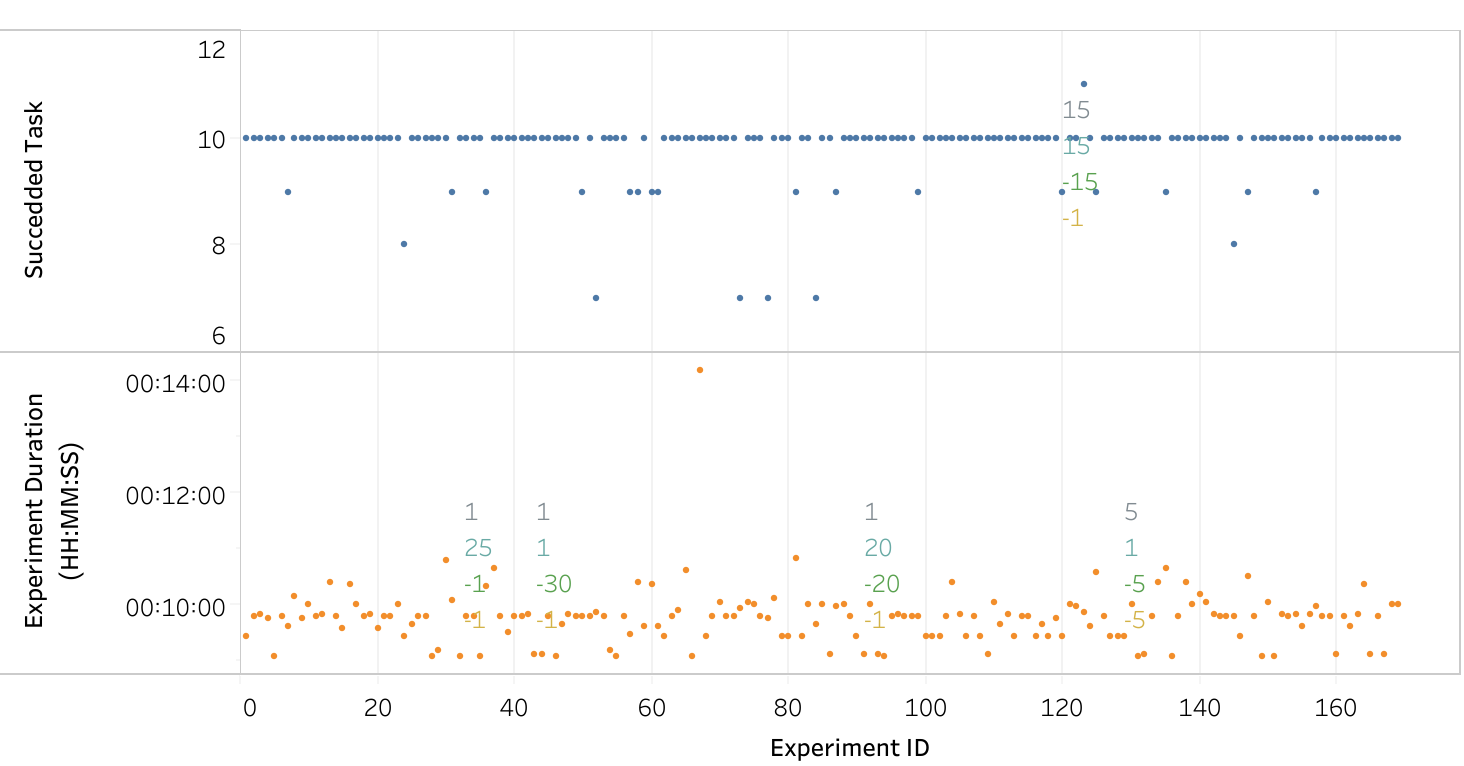
\includegraphics[width = 1.0\textwidth]{content/images/ch5/execute_experiment_30s.png}
 \caption{In each experiment, 15 ``navigation tasks'' were created with the interval of 30 seconds. The marks are labeled by weight combinations (energy consumption, waiting time, probability, priority).}
 \label{fig:experiment_task_30s}
\end{figure}

\begin{figure}[htbp]
 \centering
 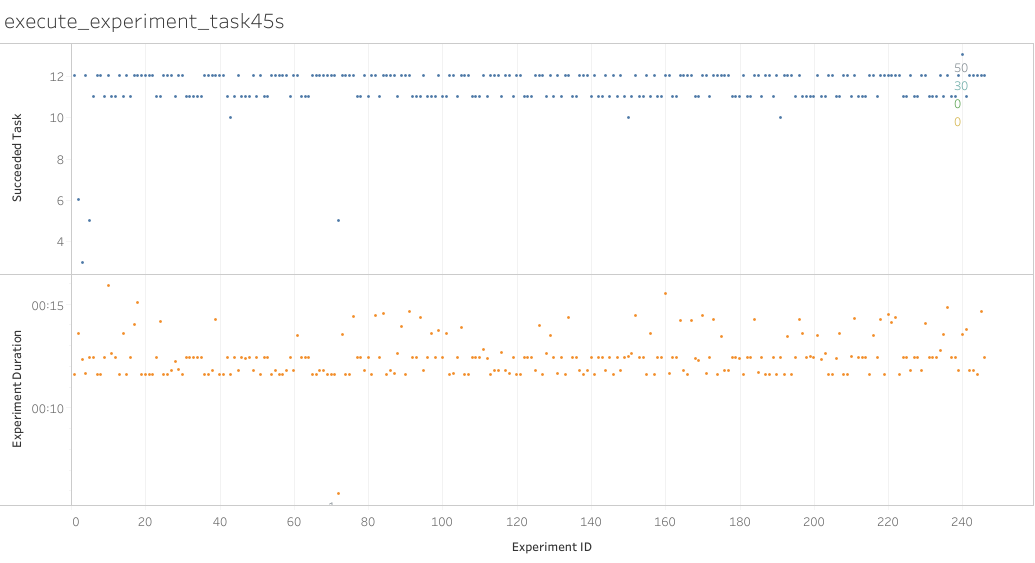
\includegraphics[width = 1.0\textwidth]{content/images/ch5/execute_experiment_45s.png}
 \caption{In each experiment, 15 ``navigation tasks'' were created with the interval of 45 seconds. The marks are labeled by weight combinations (energy consumption, waiting time, probability, priority).}
 \label{fig:experiment_task_45s}
\end{figure}

\begin{figure}[htbp]
 \centering
 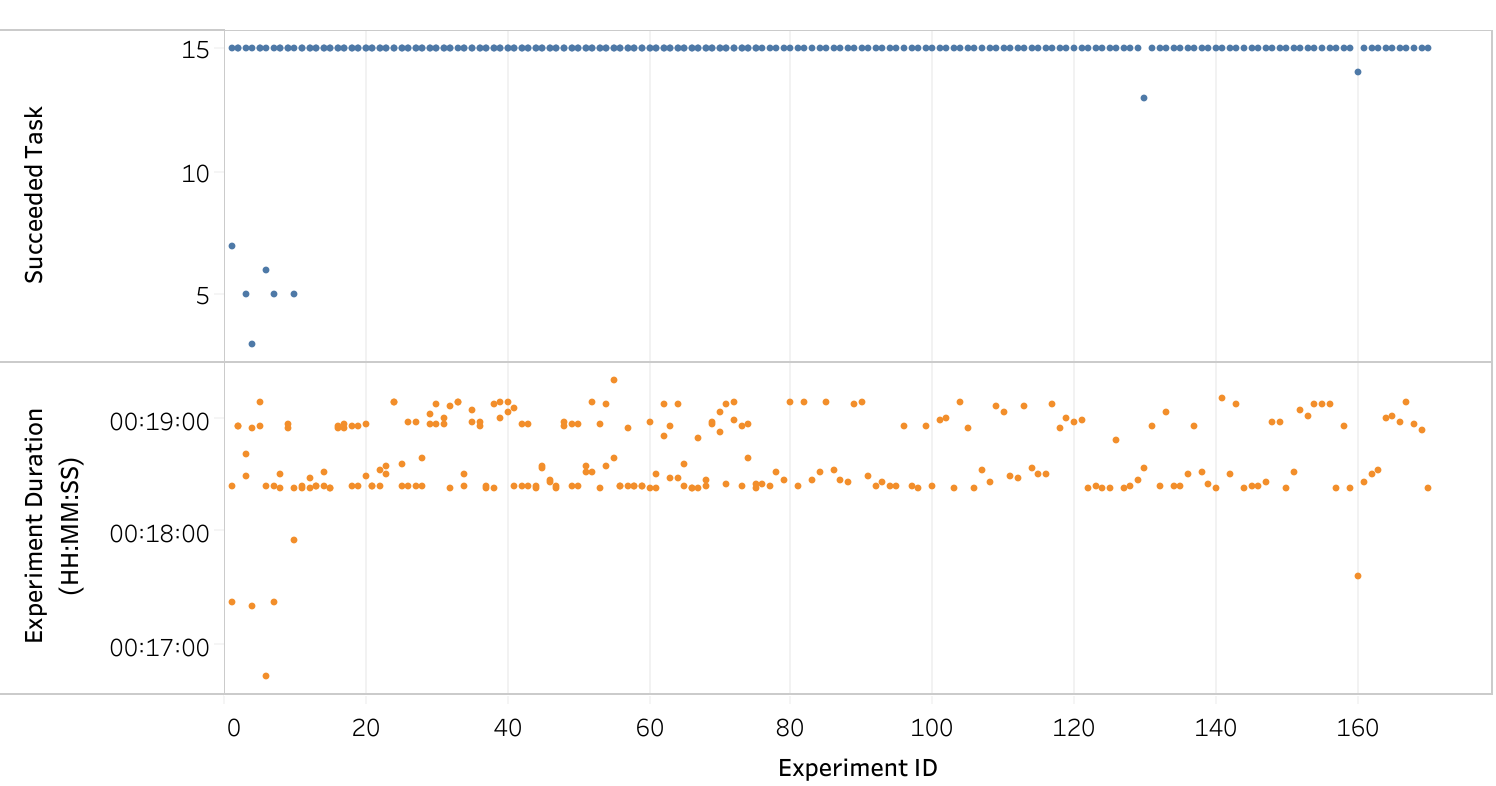
\includegraphics[width = 1.0\textwidth]{content/images/ch5/execute_experiment_65s.png}
 \caption{In each experiment, 15 ``navigation tasks'' were created with the interval of 65 seconds. The marks are labeled by weight combinations (energy consumption, waiting time, probability, priority).}
 \label{fig:experiment_task_65s}
\end{figure}

\subsection{How the Number of Robots impact task scheduling}

\paragraph{Experiment Introduction} 
In this set of experiments, how the number of robots affected task scheduling was evaluated. One of the best weight combination was selected: $ W_{\mbox{battery}} = 10,W_{\mbox{waiting time}} = 1, W_{\mbox{probability}} = -1, W_{\mbox{priority}} = -10 $. 
 


\paragraph{Analysis design}
As is discussed in the last paragraph, in each experiment, robots need to finish 15 ``navigation tasks'' and 3 ``charging tasks''.
The experiment start time was when all robot finished charging and started request task (Figure \ref{fig:execute_task_experiment_timeline}), and the experiment finish time was when the latest task is finished.
The experiment duration was an important evaluation factor, which was the time difference between the experiment start time and experiment finished time. 
The end state of ``navigation tasks'' was evaluated. In an experiment result table, the ``Succeeded'' column counted the tasks ended with ``Succeeded'' state, the ``Expired'' column counted the tasks ended with ``Succeeded'' state, the ``Failed'' column counted the tasks ended with ``Running'', ``Error'', ``Canceled'', ``To rerun'' states. 
Table \ref{tab:exp_experiment_result} is an example of experiment result. 

\paragraph{Result} The experiment result is shown in Figure \ref{fig:different_number_of_robot}.

\paragraph{Analysis} As discussed in Chapter \ref{sec:task_scheduling_procedure}, it is concluded that as the number of robots increased, the task success rate and experiment duration increased. The reason is that the robots requested tasks from the centralized pool separately. The more robots there were, the more tasks could be finished in an experiment. 
On the other hand, on average, one robot could finish 7 tasks in 17 minutes and 40 seconds, two robots could finish 11 tasks in 18 minutes and 24 seconds, and 3 robots could finish 15 tasks in 18 minutes and 52 seconds. It could be inferred that the more robots, the higher the efficiency of task scheduling.

\begin{figure}[htbp]
 \centering
 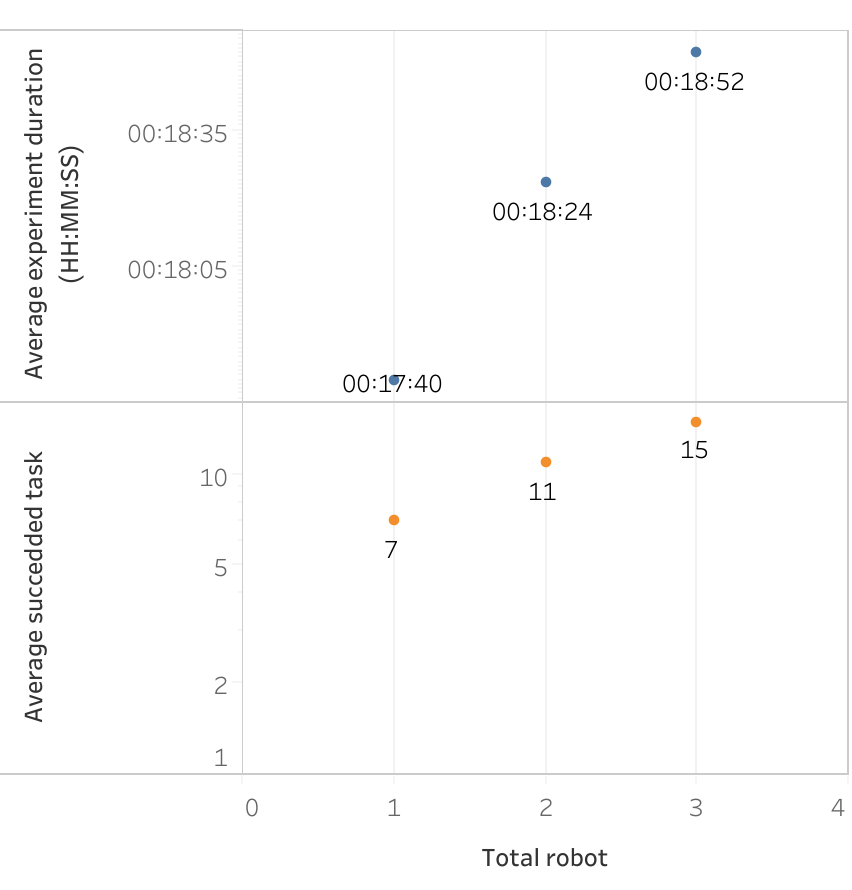
\includegraphics[width = 0.4\textwidth]{content/images/ch5/different_number_of_robots.png}
 \caption{How the number of robots impacts task scheduling}
 \label{fig:different_number_of_robot}
\end{figure}

\subsection{Evaluation of how the algorithm improves navigation tasks scheduling}

\paragraph{Experiment Introduction} 
This set of experiments evaluated how the algorithm improves the scheduling of ``navigation task''. Some experiments did not use the algorithm, and others used the designed algorithm and used the best weight combination. The experiment results will be analyzed to determine how much the designed algorithm can improve task scheduling.


\begin{figure}[htbp]
 \centering
 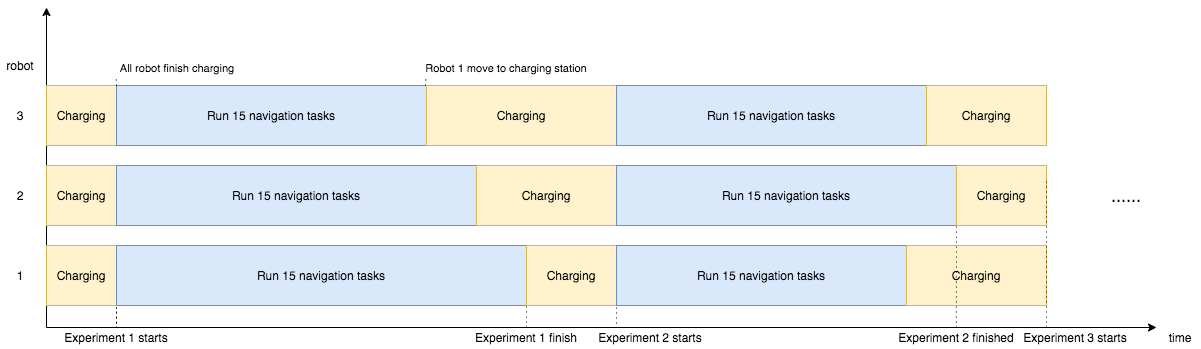
\includegraphics[width = 0.9\textwidth]{content/images/ch5/exe_exp_timeline.drawio.png}
 \caption{Execute Task Experiment Timeline}
 \label{fig:execute_task_experiment_timeline}
\end{figure}


\paragraph{Analysis design}
As is discussed in the last paragraph, in each experiment, robots need to finish 15 ``navigation tasks'' and 3 ``charging tasks''.
The experiment start time was when all robot finished charging and started request task (Figure \ref{fig:execute_task_experiment_timeline}), and the experiment finish time was when the latest task is finished.
The experiment duration was an important evaluation factor, which was the time difference between the experiment start time and experiment finished time. 
The end state of ``navigation tasks'' was evaluated. In an experiment result table, the ``Succeeded'' column counted the tasks ended with ``Succeeded'' state, the ``Expired'' column counted the tasks ended with ``Succeeded'' state, the ``Failed'' column counted the tasks ended with ``Running'', ``Error'', ``Canceled'', ``To rerun'' states. 
Table \ref{tab:exp_experiment_result} is an example of experiment result. 

\paragraph{Experiment Result} 
The experiment result is shown in Figure \ref{fig:improvement_evaluation}. In the first four experiments, the algorithm was not used because only one decision variable is considered. In the last experiment, the algorithm was used with the best weight combination.
 This experimental Result shows the difference between using the algorithm and without using the algorithm. Compared with the case that only considered the task priority, the number of successful tasks significantly increased after using the algorithm. Compared with the situation that was only waiting time are considered, all tasks were finished in both situations, but the duration of the experiment decreased. 
%The experiment result (Table \ref{tab:exp_experiment_result}.) shows that in experiment 1, all 15 tasks were successfully finished with minimal experiment duration. In experiments 2, 4, 5, more than half of the tasks was expired. In experiment 3, all tasks were successfully finished, but it took more time than experiment 1. 
The experiment 6-24 (Figure \ref{fig:only_one_decision_variable_changed}) evaluated each decision variable separately.

\begin{figure}[htbp]
 \centering
 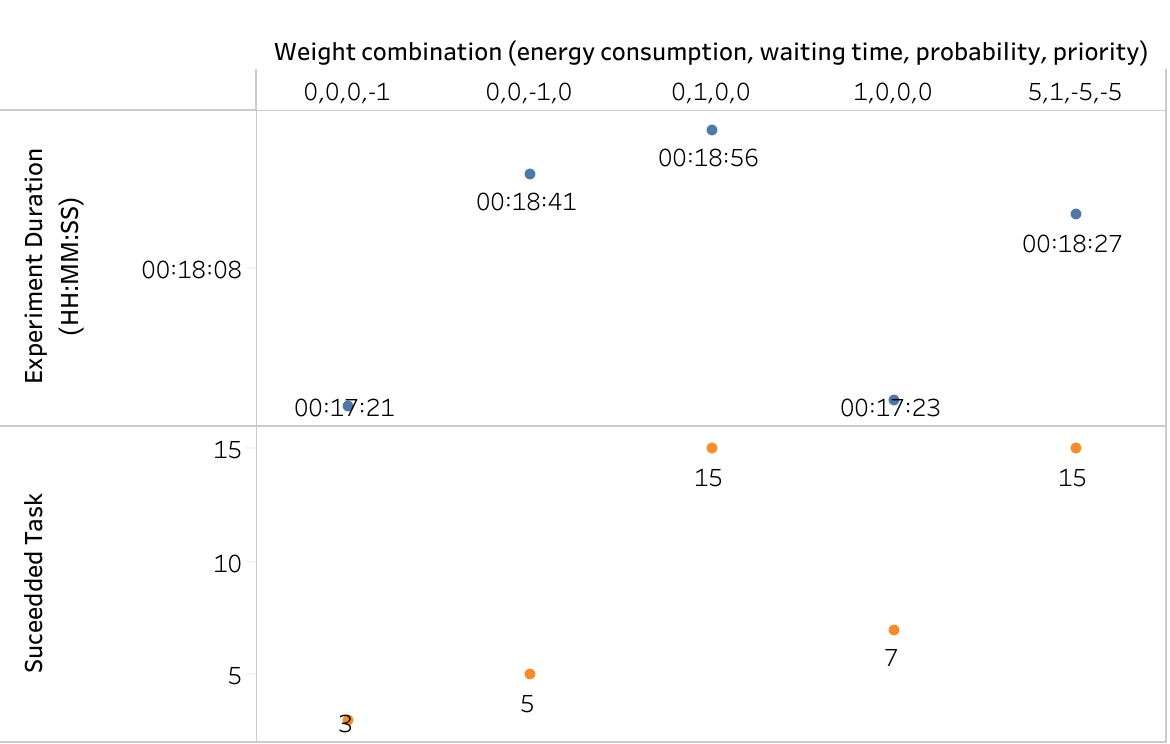
\includegraphics[width = 0.7\textwidth]{content/images/ch5/improvement_evaluation_65s.png}
 \caption{How the algorithm improves navigation task scheduling. In each experiment, 15 ``navigation tasks'' with the task interval of 65 seconds were created.}
 \label{fig:improvement_evaluation}
\end{figure}

\paragraph{Experiment Analysis.} 


The experimental results can preliminarily judge that this algorithm has a certain effect, but this effect is not particularly obvious because the simulation experiment is limited. Following are the explanation of each decision variables:

\begin{itemize}
 \item \textbf{Door Open probability.} The door open probability is used in the algorithm to make the robot more likely to go to an occupied room. As discussed in Chapter \ref{sec:limitations}, the robot can enter any room, even if its door is closed. This limitation caused the room occupancy rate not to affect the number of successful tasks and the experiment duration.
 \item \textbf{Task Priority.} Similarly, the task's priority is applied by the algorithm to allow the higher priority tasks to be executed first. However, the task priority had little effect on the experiment's two evaluation criteria: the number of successful tasks and the experiment duration. If further experiments are conducted, such as evaluating the completion of high-priority tasks, then how the priority affects task scheduling can be evaluated.
 \item \textbf{Energy consumption.} The energy consumption of the robot is considered to allow low-energy tasks to be executed first. But energy consumption had little effect on the experiment's two evaluation criteria: the number of successful tasks and the experiment duration. As discussed in Chapter \ref{sec:limitations}, the energy consumption of robots in real experiments may be accurately estimated. Then further experiments can be conducted. For example, evaluating each experiment's energy consumption, then how energy consumption affects task scheduling can be evaluated.
 \item \textbf{Waiting Time.} The task's waiting time is used in the algorithm to let the earliest tasks be executed first. As shown in Figure \ref{fig:improvement_evaluation}, the waiting time significantly optimizes task scheduling. After considering this decision variable, more tasks were successfully finished, and the experiment duration was decreased. In other words, the time required to complete all tasks was reduced. Therefore, the waiting time is a crucial decision variable in the algorithm.
\end{itemize}

\begin{figure}[htbp]
 \centering
 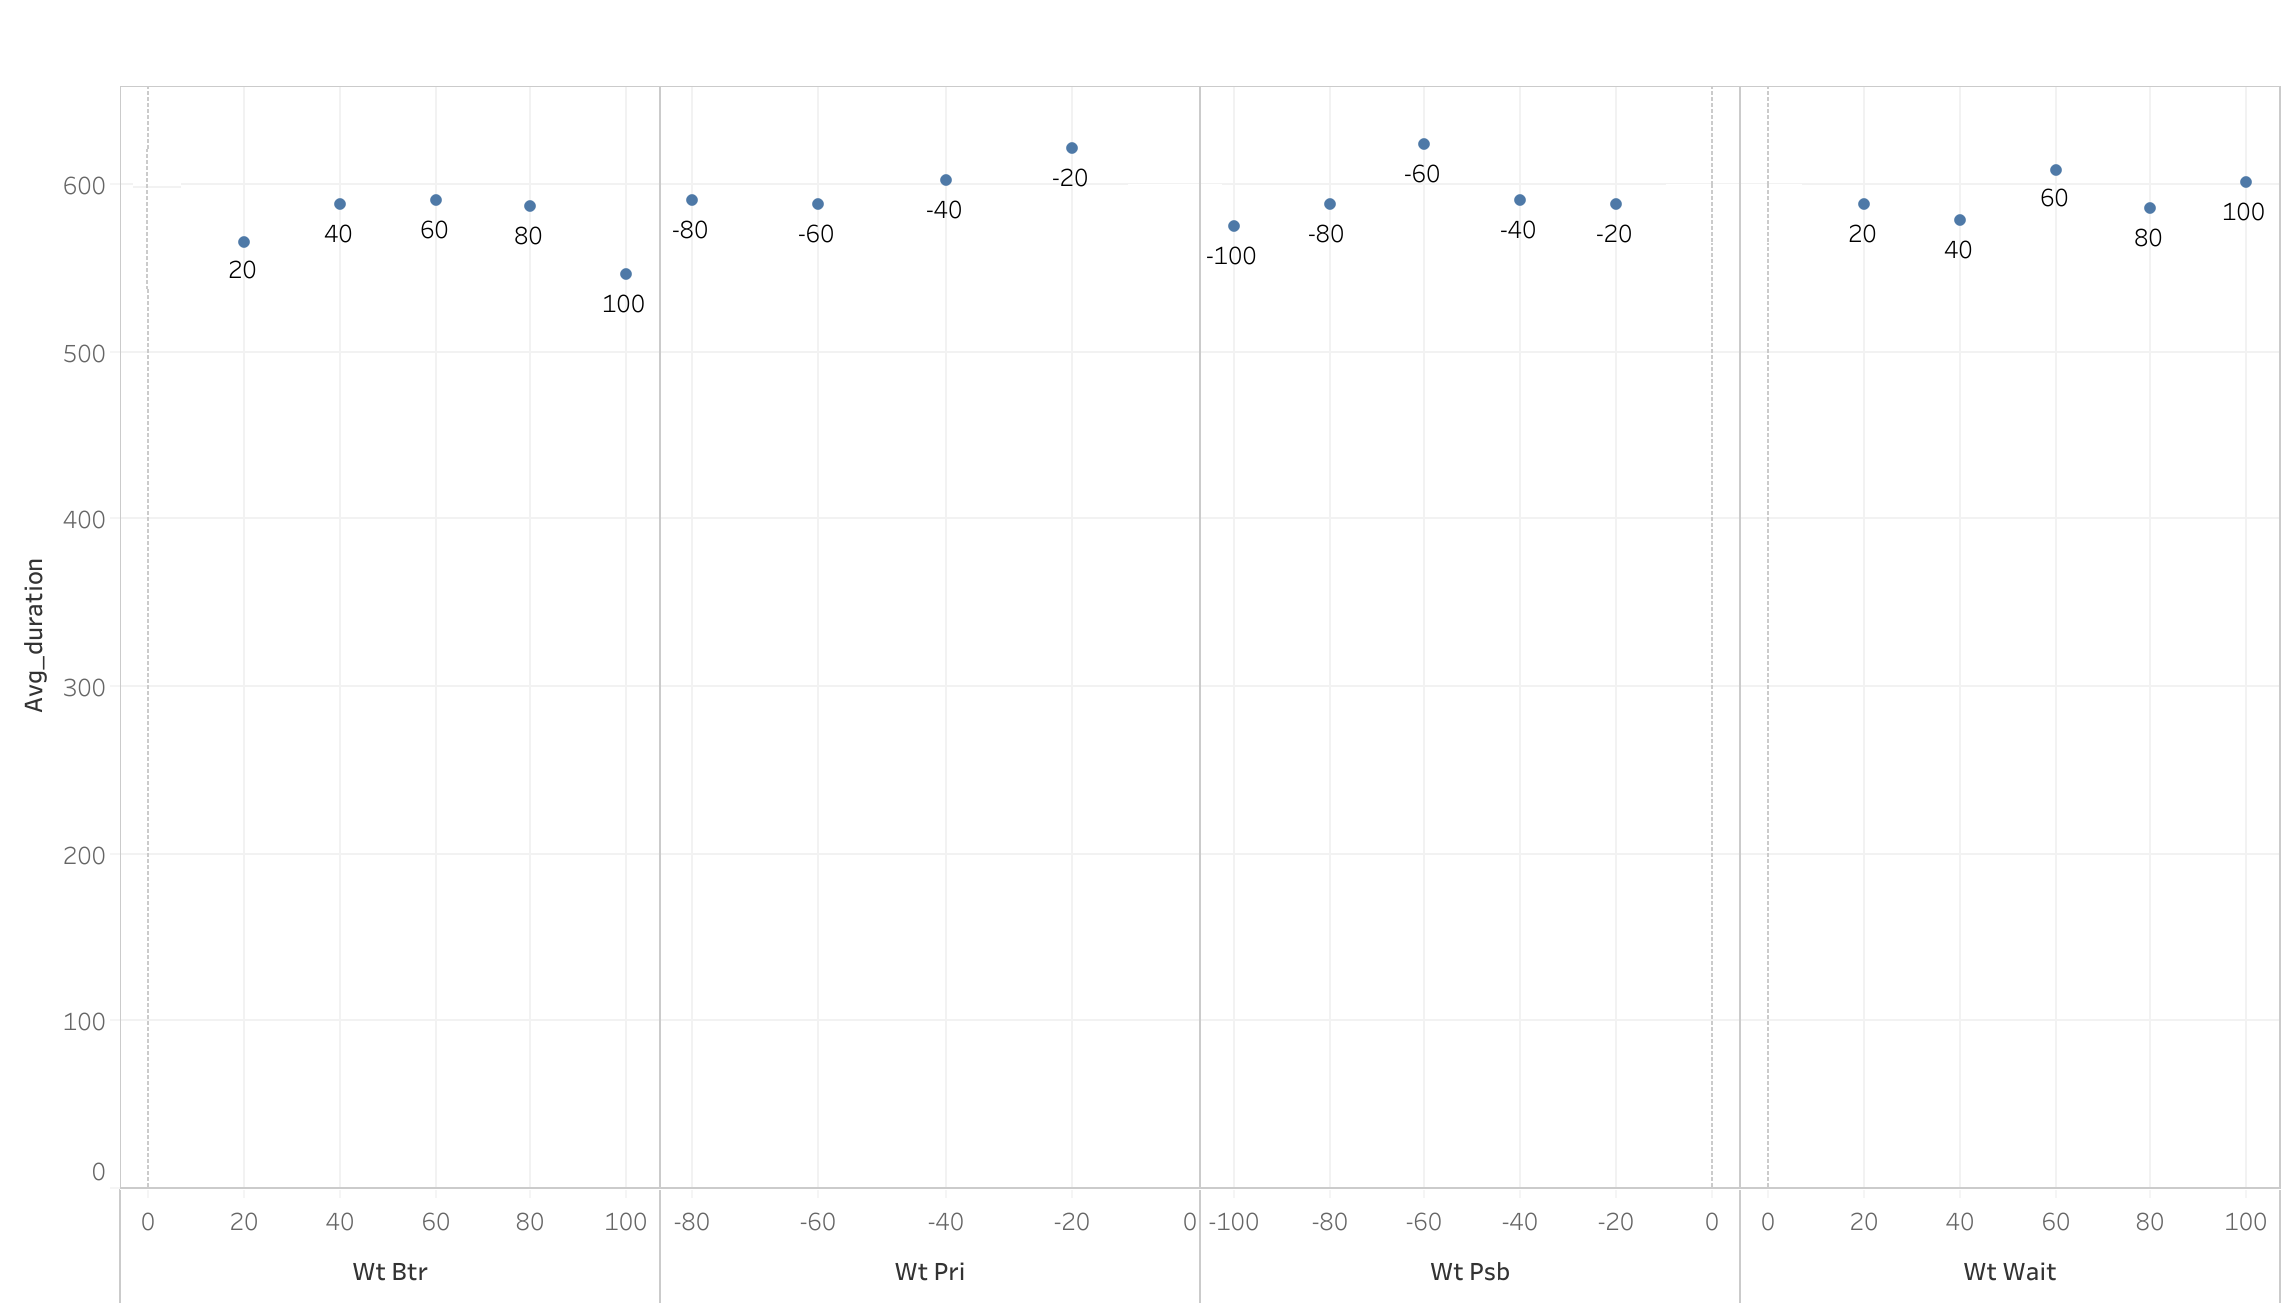
\includegraphics[width = 0.9\textwidth]{content/images/ch5/one_decision_variable.png}
 \caption{Only one decision variable changed others unchanged.}
 \label{fig:only_one_decision_variable_changed}
\end{figure}

\begin{table}[htb]
\centering
\resizebox{\textwidth}{!}{
\begin{tabular}{|c|c|c|c|c|c|c|c|c|c|c|c|} 
\hline
Experiment & $W_{\mbox{battery}}$ & $W_{\mbox{waiting time}}$ & $W_{\mbox{door open probability}}$ & $W_{\mbox{priority}}$ & Experiment Duration &Total Task & Succedded Task & Expired Task & Failed Task \\
\hline
1 & 1.00 & 1.00 & -1.00& -1.00& 00:18:23 & 15 & 15 & 0 & 0 \\\hline
2 & 1.00 & 0.00 & 0.00 & 0.00 & 00:17:23 & 15 & 7 & 8 & 0 \\ \hline
3 & 0.00 & 1.00 & 0.00 & 0.00 & 00:18:56 & 15 & 15 & 0 & 0 \\\hline
4 & 0.00 & 0.00 & -1.00 & 0.00 & 00:18:41 & 15 & 5 & 10 & 0 \\\hline 
5 & 0.00 & 0.00 & 0.00 & -1.00& 00:17:21 & 15 & 3 & 12 & 0 \\ \hline
\end{tabular}}
\caption{Example experiment result.}
\label{tab:exp_experiment_result}
\end{table}


\begin{table}[]
\resizebox{\textwidth}{!}{
\begin{tabular}{|c|c|c|c|c|c|c|c|c|c|}
\hline
Task ID & Task Name & Start Time & Target ID & Robot ID &Priority & Task Status & Dependency & Finish Time & Description \\ \hline
1 & Charging & NULL & 18 & 1 & 5 & Succedded & 0 & 2020-06-02 11:03:12 & Succeeded \\ \hline
2 & Charging & NULL & 19 & 2 & 5 & Succedded & 0 & 2020-06-02 11:03:12 & Succeeded \\ \hline
3 & Charging & NULL & 20 & 3 & 5 & Succedded & 0 & 2020-06-02 11:03:11 & Succeeded \\ \hline
4 & Navigation & 2020-06-02 11:04:17 & 21 & 3 & 2 & Succedded & 0 & 2020-06-02 11:05:16 & Succeeded \\ \hline
5 & Navigation & 2020-06-02 11:05:22 & 22 & 1 & 2 & Succedded & 0 & 2020-06-02 11:07:29 & Succeeded \\ \hline
6 & Navigation & 2020-06-02 11:06:27 & 23 & 2 & 2 & Succedded & 0 & 2020-06-02 11:08:06 & Succeeded \\ \hline
7 & Navigation & 2020-06-02 11:07:32 & 24 & 3 & 2 & Succedded & 0 & 2020-06-02 11:09:25 & Succeeded \\ \hline
8 & Navigation & 2020-06-02 11:08:37 & 25 & 1 & 2 & Succedded & 0 & 2020-06-02 11:10:46 & Succeeded \\ \hline
9 & Navigation & 2020-06-02 11:09:42 & 26 & 2 & 2 & Succedded & 0 & 2020-06-02 11:12:42 & Succeeded \\ \hline
10 & Navigation & 2020-06-02 11:10:47 & 27 & 3 & 2 & Succedded & 0 & 2020-06-02 11:12:56 & Succeeded \\ \hline
11 & Navigation & 2020-06-02 11:11:52 & 28 & 1 & 2 & Succedded & 0 & 2020-06-02 11:14:13 & Succeeded \\ \hline
12 & Navigation & 2020-06-02 11:12:57 & 29 & 2 & 2 & Succedded & 0 & 2020-06-02 11:14:20 & Succeeded \\ \hline
13 & Navigation & 2020-06-02 11:14:02 & 30 & 3 & 2 & Succedded & 0 & 2020-06-02 11:15:36 & Succeeded \\ \hline
14 & Navigation & 2020-06-02 11:15:07 & 21 & 1 & 2 & Succedded & 0 & 2020-06-02 11:18:07 & Succeeded \\ \hline
15 & Navigation & 2020-06-02 11:16:12 & 22 & 2 & 2 & Succedded & 0 & 2020-06-02 11:18:49 & Succeeded \\ \hline
16 & Navigation & 2020-06-02 11:17:17 & 23 & 3 & 2 & Succedded & 0 & 2020-06-02 11:18:58 & Succeeded \\ \hline
17 & Navigation & 2020-06-02 11:18:22 & 24 & 1 & 2 & Succedded & 0 & 2020-06-02 11:20:14 & Succeeded \\ \hline
18 & Navigation & 2020-06-02 11:19:27 & 25 & 2 & 2 & Succedded & 0 & 2020-06-02 11:21:36 & Succeeded \\ \hline
19 & Charging & NULL & 18 & 1 & 5 & Succedded & 0 & 2020-06-02 11:23:08 & Succeeded \\ \hline
20 & Charging & NULL & 19 & 2 & 5 & Succedded & 0 & 2020-06-02 11:23:08 & Succeeded \\ \hline
21 & Charging & NULL & 20 & 3 & 5 & Succedded & 0 & 2020-06-02 11:23:08 & Succeeded \\ \hline
22 & Navigation & 2020-06-02 11:24:13 & 21 & 3 & 2 & Succedded & 0 & 2020-06-02 11:25:12 & Succeeded \\ \hline
23 & Navigation & 2020-06-02 11:25:18 & 22 & 2 & 2 & Succedded & 0 & 2020-06-02 11:26:54 & Succeeded \\ \hline
24 & Navigation & 2020-06-02 11:26:23 & 23 & 1 & 2 & Succedded & 0 & 2020-06-02 11:28:35 & Succeeded \\ \hline
25 & Navigation & 2020-06-02 11:27:28 & 24 & 3 & 2 & Succedded & 0 & 2020-06-02 11:29:23 & Succeeded \\ \hline
26 & Navigation & 2020-06-02 11:28:33 & 25 & 2 & 2 & Succedded & 0 & 2020-06-02 11:30:41 & Succeeded \\ \hline
27 & Navigation & 2020-06-02 11:29:38 & 26 & 1 & 2 & Succedded & 0 & 2020-06-02 11:32:37 & Succeeded \\ \hline
28 & Navigation & 2020-06-02 11:30:43 & 27 & 3 & 2 & Succedded & 0 & 2020-06-02 11:32:54 & Succeeded \\ \hline
29 & Navigation & 2020-06-02 11:31:48 & 28 & 2 & 2 & Succedded & 0 & 2020-06-02 11:34:09 & Succeeded \\ \hline
30 & Navigation & 2020-06-02 11:32:53 & 29 & 1 & 2 & Succedded & 0 & 2020-06-02 11:34:15 & Succeeded \\ \hline
31 & Navigation & 2020-06-02 11:33:58 & 30 & 3 & 2 & Succedded & 0 & 2020-06-02 11:35:32 & Succeeded \\ \hline
32 & Navigation & 2020-06-02 11:35:03 & 21 & 2 & 2 & Succedded & 0 & 2020-06-02 11:38:03 & Succeeded \\ \hline
33 & Navigation & 2020-06-02 11:36:08 & 22 & 1 & 2 & Succedded & 0 & 2020-06-02 11:38:45 & Succeeded \\ \hline
34 & Navigation & 2020-06-02 11:37:13 & 23 & 3 & 2 & Succedded & 0 & 2020-06-02 11:38:54 & Succeeded \\ \hline
35 & Navigation & 2020-06-02 11:38:18 & 24 & 2 & 2 & Succedded & 0 & 2020-06-02 11:40:11 & Succeeded \\ \hline
36 & Navigation & 2020-06-02 11:39:23 & 25 & 1 & 2 & Succedded & 0 & 2020-06-02 11:41:40 & Succeeded \\ \hline
37 & Charging & NULL & 18 & 1 & 5 & Succedded & 0 & 2020-06-02 11:43:45 & Succeeded \\ \hline
38 & Charging & NULL & 19 & 2 & 5 & Succedded & 0 & 2020-06-02 11:43:45 & Succeeded \\ \hline
39 & Charging & NULL & 20 & 3 & 5 & Succedded & 0 & 2020-06-02 11:43:45 & Succeeded \\ \hline
\end{tabular}}
\caption{Task Table}
\label{tab:exp_task_table}
\end{table}


% \begin{table}[htb]
% \centering
% \resizebox{\textwidth}{!}{
% \begin{tabular}{|c|c|c|c|c|c|c|c|c|c|c|c|} 
% \hline
% $W_{\mbox{battery}}$ & $W_{\mbox{waiting time}}$ & $W_{\mbox{door probability}}$ & $W_{\mbox{priority}}$ & Experiment Duration &Total Task & Succedded Task & Expired Task & Failed Task \\
% \hline
% 1 & 1 & -1 & -10 & 00:11:35 & 15 & 12 & 3 & 0 \\ \hline
% 1 & 50 & -50 & -50 & 00:11:35 & 15 & 12 & 3 & 0 \\ \hline
% 25 & 20 & 0 & 0 & 00:11:35 & 15 & 12 & 3 & 0 \\ \hline
% 35 & 30 & 0 & 0 & 00:11:35 & 15 & 12 & 3 & 0 \\ \hline
% 40 & 10 & 0 & 0 & 00:11:35 & 15 & 12 & 3 & 0 \\ \hline
% 45 & 1 & -1 & -1 & 00:11:35 & 15 & 12 & 3 & 0 \\ \hline
% 50 & 50 & -50 & -1 & 00:11:35 & 15 & 12 & 3 & 0 \\ \hline
% \end{tabular}}
% \caption{Best weight combinations with task time interval 45s.}
% \label{tab:exp_task_45s}
% \end{table}


% \begin{table}[htb]
 % \centering
 % \resizebox{\textwidth}{!}{
 % \begin{tabular}{|c|c|c|c|c|c|c|c|c|c|c|c|} 
 % \hline
 % $W_{\mbox{battery}}$ & $W_{\mbox{waiting time}}$ & $W_{\mbox{door probability}}$ & $W_{\mbox{priority}}$ & Experiment Duration &Total Task & Succedded Task & Expired Task & Failed Task \\
 % \hline
 % 1 & 1 & -1 & -3 & 00:09:05 & 15 & 10 & 5 & 0 \\ \hline
 % 1 & 1 & -30 & -1 & 00:09:05 & 15 & 10 & 5 & 0 \\ \hline
 % 1 & 20& -20 & -1 & 00:09:05 & 15 & 10 & 5 & 0 \\ \hline
 % 1 & 25& -1 & -1 & 00:09:05 & 15 & 10 & 5 & 0 \\ \hline
 % 5 & 1 & -5 & -5 & 00:09:05 & 15 & 10 & 5 & 0 \\ \hline
 % \end{tabular}}
 % \caption{Best weight combinations with task time interval 30s.}
 % \label{tab:exp_task_30s}
 % \end{table}
 
 
% \begin{table}[]
% \resizebox{\textwidth}{!}{
% \begin{tabular}{|l|l|l|l|l|l|l|l|l|l|}
% \hline
% Experiment & $W_{\mbox{battery}}$ & $W_{\mbox{waiting time}}$ & $W_{\mbox{door probability}}$ & $W_{\mbox{priority}}$ & Experiment Duration &Total Task & Succeeded Task & Expired Task & Failed Task \\ \hline
% 6 & 20 & 1 & -1 & -1 & 00:09:26 & 15 & 10 & 5 & 0 \\ \hline
% 7 & 40 & 1 & -1 & -1 & 00:09:48 & 15 & 10 & 5 & 0 \\ \hline
% 8 & 60 & 1 & -1 & -1 & 00:09:50 & 15 & 10 & 5 & 0 \\ \hline
% 9 & 80 & 1 & -1 & -1 & 00:09:47 & 15 & 10 & 5 & 0 \\ \hline
% 10 & 100 & 1 & -1 & -1 & 00:09:06 & 15 & 10 & 5 & 0 \\ \hline
% 11 & 1 & 20 & -1 & -1 & 00:09:48 & 15 & 10 & 5 & 0 \\ \hline
% 12 & 1 & 40 & -1 & -1 & 00:09:38 & 15 & 9 & 5 & 0 \\ \hline
% 13 & 1 & 60 & -1 & -1 & 00:10:09 & 15 & 10 & 5 & 0 \\ \hline
% 14 & 1 & 80 & -1 & -1 & 00:09:46 & 15 & 10 & 5 & 0 \\ \hline
% 15 & 1 & 100 & -1 & -1 & 00:10:01 & 15 & 10 & 5 & 0 \\ \hline
% 16 & 1 & 1 & -20 & -1 & 00:09:48 & 15 & 10 & 5 & 0 \\ \hline
% 17 & 1 & 1 & -40 & -1 & 00:09:50 & 15 & 10 & 5 & 0 \\ \hline
% 18 & 1 & 1 & -60 & -1 & 00:10:24 & 15 & 10 & 5 & 0 \\ \hline
% 19 & 1 & 1 & -80 & -1 & 00:09:48 & 15 & 10 & 5 & 0 \\ \hline
% 20 & 1 & 1 & -100 & -1 & 00:09:35 & 15 & 10 & 5 & 0 \\ \hline
% 21 & 1 & 1 & -1 & -20 & 00:10:22 & 15 & 10 & 5 & 0 \\ \hline
% 22 & 1 & 1 & -1 & -40 & 00:10:02 & 15 & 10 & 5 & 0 \\ \hline
% 23 & 1 & 1 & -1 & -60 & 00:09:48 & 15 & 10 & 5 & 0 \\ \hline
% 24 & 1 & 1 & -1 & -80 & 00:09:51 & 15 & 10 & 5 & 0 \\ \hline
% \end{tabular}}
% \caption{only one decision variable changed others unchanged.}
% \label{tab:only_one_decision_variable_changed}
% \end{table}



% \begin{table}[htb]
% \centering
% \resizebox{\textwidth}{!}{
% \begin{tabular}{|c|c|c|c|c|c|c|c|c|c|c|c|} 
% \hline
% $W_{\mbox{battery}}$ & $W_{\mbox{waiting time}}$ & $W_{\mbox{door probability}}$ & $W_{\mbox{priority}}$ & Experiment Duration &Total Task & Succedded Task & Expired Task & Failed Task \\
% \hline
% 10.00 & 1.00 & -1.00 & 0.00 & 00:18:23 & 15 & 15 & 0 & 0 \\ \hline
% 1.00 & 1.00 & -1.00 & 0.00 & 00:18:23 & 15 & 15 & 0 & 0 \\ \hline
% 1.00 & 1.00 & -1.00 & -1.00 & 00:18:23 & 15 & 15 & 0 & 0 \\ \hline
% 1.00 & 5.00 & -1.00 & -1.00 & 00:18:23 & 15 & 15 & 0 & 0 \\ \hline
% 1.00 & 5.00 & -1.00 & -5.00 & 00:18:23 & 15 & 15 & 0 & 0 \\ \hline
% 1.00 & 10.00 & -10.00 & -1.00 & 00:18:23 & 15 & 15 & 0 & 0 \\ \hline
% 1.00 & 5.00 & -5.00 & -5.00 & 00:18:23 & 15 & 15 & 0 & 0 \\ \hline
% 1.00 & 5.00 & -10.00 & -5.00 & 00:18:23 & 15 & 15 & 0 & 0 \\ \hline
% 1.00 & 5.00 & -1.00 & -1.00 & 00:18:23 & 15 & 15 & 0 & 0 \\ \hline
% 1.00 & 20.00 & -1.00 & -1.00 & 00:18:23 & 15 & 15 & 0 & 0 \\ \hline
% 1.00 & 1.00 & -1.00 & -30.00 & 00:18:23 & 15 & 15 & 0 & 0 \\ \hline
% 1.00 & 1.00 & -1.00 & -35.00 & 00:18:23 & 15 & 15 & 0 & 0 \\ \hline
% 10.00 & 1.00 & -1.00 & -5.00 & 00:18:23 & 15 & 15 & 0 & 0 \\ \hline
% 10.00 & 10.00 & -1.00 & -1.00 & 00:18:23 & 15 & 15 & 0 & 0 \\ \hline
% 10.00 & 1.00 & -1.00 & -1.00 & 00:18:23 & 15 & 15 & 0 & 0 \\ \hline
% 10.00 & 1.00 & -10.00 & -1.00 & 00:18:23 & 15 & 15 & 0 & 0 \\ \hline
% 10.00 & 5.00 & -5.00 & -5.00 & 00:18:23 & 15 & 15 & 0 & 0 \\ \hline
% 10.00 & 1.00 & -10.00 & -5.00 & 00:18:23 & 15 & 15 & 0 & 0 \\ \hline
% 10.00 & 10.00 & -10.00 & -10.00 & 00:18:23 & 15 & 15 & 0 & 0 \\ \hline
% 10.00 & 1.00 & -10.00 & -1.00 & 00:18:23 & 15 & 15 & 0 & 0 \\ \hline
% 25.00 & 1.00 & -1.00 & -25.00 & 00:18:23 & 15 & 15 & 0 & 0 \\ \hline
% 30.00 & 30.00 & -1.00 & -1.00 & 00:18:23 & 15 & 15 & 0 & 0 \\ \hline
% 45.00 & 1.00 & -1.00 & -1.00 & 00:18:23 & 15 & 15 & 0 & 0 \\ \hline
% 45.00 & 1.00 & -45.00 & -1.00 & 00:18:23 & 15 & 15 & 0 & 0 \\ \hline
% 5.00 & 10.00 & -10.00 & -1.00 & 00:18:23 & 15 & 15 & 0 & 0 \\ \hline
% 5.00 & 5.00 & -1.00 & -1.00 & 00:18:23 & 15 & 15 & 0 & 0 \\ \hline
% 5.00 & 10.00 & -5.00 & -1.00 & 00:18:23 & 15 & 15 & 0 & 0 \\ \hline
% 5.00 & 5.00 & -10.00 & -1.00 & 00:18:23 & 15 & 15 & 0 & 0 \\ \hline
% 5.00 & 10.00 & -10.00 & -1.00 & 00:18:23 & 15 & 15 & 0 & 0 \\ \hline
% 5.00 & 5.00 & -1.00 & -5.00 & 00:18:23 & 15 & 15 & 0 & 0 \\ \hline
% 5.00 & 10.00 & -5.00 & -10.00 & 00:18:23 & 15 & 15 & 0 & 0 \\ \hline
% \end{tabular}}
% \caption{Best weight combinations with task time interval 65s.}
% \label{tab:exp_task_65s}
% \end{table}

